\chapter{Reject Inference} \label{chap2}

\epigraph{Sounds good, doesn't work.}{Donald J.\ Trump}

\textit{Nota Bene :} ce chapitre s'inspire fortement de l'article [...]

\selectlanguage{english}

The granting process of all credit institutions rejects applicants who seem risky regarding the repayment of their debt. A credit score is calculated and associated with a cut-off value beneath which an applicant is rejected. Developing a new scorecard, i.e. a correspondence table between a client's characteristics and his/her score, implies having a learning dataset in which the response variable good/bad borrower is known, so that rejects are \textit{de facto} excluded from the learning process. It might have deep consequences on the scorecard relevance as the learning population has been financed and considered good by the previous model. Previous works from the literature in this matter consisted mostly in empirical methods to exploit rejected applicants' data in the scorecard development process and experiments. We propose a rational criterion to evaluate the quality of a scoring model. We review each existing method in light of our criterion and dig out their implicit mathematical hypotheses. We show that up to now, no \textit{Reject Inference} method can guarantee to provide an improved credit scorecard. To support these theoretical findings, we added experiments on simulated and real data from the french branch of Crédit Agricole Consumer Finance.



\section{}



\begin{figure}[ht]
\begin{minipage}[b]{0.45\linewidth}
\center 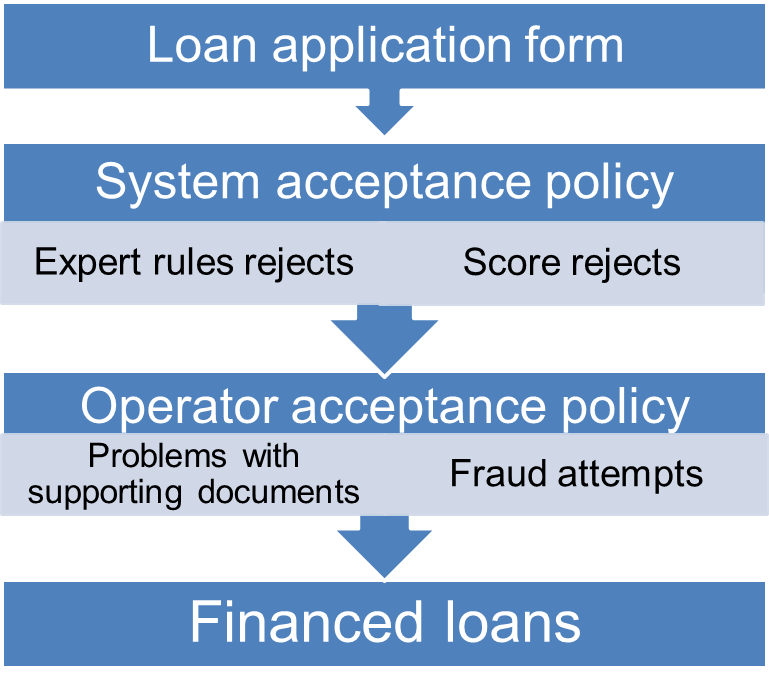
\includegraphics[width=5cm]{figures/chapitre2/schema.png}
\caption{Simplified Acceptance mechanism in~Crédit Agricole Consumer Finance}
\label{fig:figure1}

\end{minipage}%
\hfil \begin{minipage}[b]{0.5\linewidth}

\center 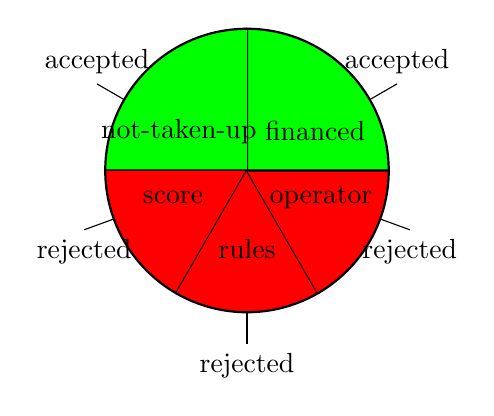
\begin{tikzpicture}

    \foreach \start/\end/\middle/\percent/\anchor/\name in {
      0/90/30/financed/above/accepted,
      90/180/150/not-taken-up/above/accepted}
  {
    \draw[fill=green, thick] (0,0) -- (\end:1.8cm) arc (\end:\start:1.8cm)
      node at (\middle:1cm) {\percent};
    \draw (\middle:1.8cm) -- (\middle:2.2cm) node[\anchor] {\name};
  };
    
    \foreach \start/\end/\middle/\percent/\anchor/\name in {
      180/240/200/score/below/rejected,
      240/300/270/rules/below/rejected,
      300/360/340/operator/below/rejected}
  {
    \draw[fill=red, thick] (0,0) -- (\end:1.8cm) arc (\end:\start:1.8cm)
      node at (\middle:1cm) {\percent};
    \draw (\middle:1.8cm) -- (\middle:2.2cm) node[\anchor] {\name};
  };
\end{tikzpicture}
\caption{Simplified Acceptance status in Crédit Agricole Consumer Finance - scale relations not respected}
\label{fig:figure2}

\end{minipage}
\end{figure}



\printbibliography[heading=subbibliography, title=References of Chapter 2]